\documentclass{article}[10pt]

%\usepackage{fullpage}

\usepackage[english]{babel}
\usepackage{microtype}
\usepackage{graphicx}
\usepackage{caption}
\usepackage{subcaption} \usepackage{hyperref}


\title{Scientific Visualization and Virtual Reality – Exercise 4}
\author{Maarten Inja (5872464) \& Chiel Kooijman (5743028)}

\begin{document}
\maketitle

In this report we describe how we have visualized a frog. We have been given two
processed datasets: one with the exterior (skin) of a frog, and one with the
intestines. The latter set was separated; each organ had an index.

We used VTK to create a visualization. The datatype was given in the
assignment, and so it was not difficult to read the data. We used the index of an
organ throughout our program to specific the color in the representation,
whether an organ should be rendered, and the opacity of organs.

A standard \emph{vtkRenderWindowInteractor} was implemented to enable the default
vtk interaction behaviour of the visualisation. Furthermore, we created a class
which extends the \emph{vtkInteractorStyleTrackballCamera} in order to catch
mouse events. This class enabled us to check if a user presses on organ name in
the legend and subsequently disable or renable the rendering of the selected
organ.

In the process of selecting the colors for the organs we balanced between our
goal of choosing colors that are realistic (i.e. the expected color of the organ
in real frogs) and our goal of creating a rendering in which it is easy to
recognize different organs.

Figure \ref{fig:frog_brain} shows our visualisation in which only the eye retina,
eye white, the brain and the nerves are rendered. The legend can be seen in the
bottom left corner. Note that it is not possible to toggle the rendering of the
frog skin, this is always rendered.

\begin{figure}[h]
    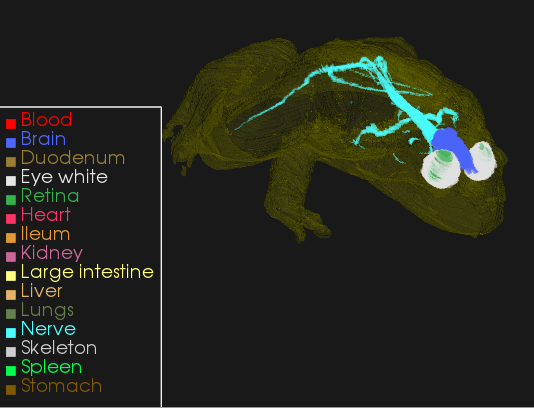
\includegraphics[width=\textwidth]{frog_brain}
    \caption{Our visualization depicting the with the eye retina, eye white, the brain and the nerves.}
    \label{fig:frog_brain}
\end{figure}

Our code can be downloaded from our github repository:
\url{https://github.com/chielk/beautiful\_data}.



\end{document}
